%%%%%%%%%%%%%%%%%%%%%%%%%%%%%%%%%%%%%%%%%%%%%%
% Lab report template.
%%%%%%%%%%%%%%%%%%%%%%%%%%%%%%%%%%%%%%%%%%%%%%

\documentclass[aps,letterpaper,10pt]{revtex4}

\usepackage{subfigure}
\usepackage{wrapfig}
\usepackage{graphicx} % For images
\usepackage{float}    % For tables and other floats
\usepackage{verbatim} % For comments and other
\usepackage{amsmath}  % For math
\usepackage{amssymb}  % For more math
\usepackage{fullpage} % Set margins and place page numbers at bottom center
\usepackage{listings} % For source code
\usepackage{subfig}   % For subfigures
\usepackage[usenames,dvipsnames]{color} % For colors and names
%\usepackage[section]{placeins}


\definecolor{mygrey}{gray}{.96} % Light Grey
\lstset{ 
    language= Matlab,               % choose the language of the code ("language=Verilog" is %popular as well)
    tabsize=3,    					% sets the size of the tabs in spaces (1 Tab %is replaced with 3 spaces)
	basicstyle=\tiny,               % the size of the fonts that are used for the code
	numbers=left,                   % where to put the line-numbers
	numberstyle=\tiny,              % the size of the fonts that are used for the line-numbers
	stepnumber=2,                   % the step between two line-numbers. If it's 1 each line will %be numbered
	numbersep=5pt,                  % how far the line-numbers are from the code
	backgroundcolor=\color{mygrey}, % choose the background color. You must add %\usepackage{color}
	frame=single,	                % adds a frame around the code
	tabsize=3,	                    % sets default tabsize to 2 spaces
	captionpos=b,                   % sets the caption-position to bottom
	breaklines=true,                % sets automatic line breaking
	breakatwhitespace=false,        % sets if automatic breaks should only happen at whitespace
	%escapeinside={\%*}{*)},        % if you want to add a comment within your code
	commentstyle=\color{BrickRed}   % sets the comment style
}



% TITLE PAGE CONTENT %%%%%%%%%%%%%%%%%%%%%%%%
% Remember to fill this section out for each
% lab write-up.
%%%%%%%%%%%%%%%%%%%%%%%%%%%%%%%%%%%%%%%%%%%%%
\newcommand{\labno}{02}
\newcommand{\labtitle}{Factory Simulation}
\newcommand{\authorname}{Ahmed Kotb (11), Ahmed Mohsen (14), Amr Sharaf (42)}
\newcommand{\professor}{Dr.Sahar Ghanem, Eng.Ahmed Essam}
\newcommand{\classno}{CS433: Performance Evaluation}
% END TITLE PAGE CONTENT %%%%%%%%%%%%%%%%%%%%

% Make units a little nicer looking and faster to type
\newcommand{\Hz}{\textsl{Hz}}
\newcommand{\KHz}{\textsl{KHz}}
\newcommand{\MHz}{\textsl{MHz}}
\newcommand{\GHz}{\textsl{GHz}}
\newcommand{\ns}{\textsl{ns}}
\newcommand{\ms}{\textsl{ms}}
\newcommand{\s}{\textsl{s}}

\begin{document}  % START THE DOCUMENT!


% TITLE PAGE %%%%%%%%%%%%%%%%%%%%%%%%%%%%%%%%%%%%%%
% If you'd like to change the content of this,
% do it in the "TITLE PAGE CONTENT" directly above
% this message
%%%%%%%%%%%%%%%%%%%%%%%%%%%%%%%%%%%%%%%%%%%%%%%%%%%
\begin{titlepage}
\begin{center}

\includegraphics[width=2cm]{Logo_Alexandria_University.jpg}\\
{\LARGE \textsc{Assignment No. \labno:} \\ \vspace{4pt}}
{\Large \textsc{\labtitle} \\ \vspace{4pt}} 
\rule[13pt]{\textwidth}{1pt} \\ \vspace{150pt}
{\large By: \authorname \\ \vspace{10pt}
Instructors: \professor \\ \vspace{10pt}
\classno \\ \vspace{10pt}
\today}
\end{center}
\end{titlepage}
% END TITLE PAGE %%%%%%%%%%%%%%%%%%%%%%%%%%%%%%%%%%
\tableofcontents
\newpage
%\listoffigures
%\newpage


%%%%%%%%%%%%%%%%%%%%%%%%%%%%%%
%%%%%%%%%%%%%%%%%%%%%%%%%%%%%%
\section{Introduction}
%No Text Here
%%%%%%%%%%%%%%%%%%%%%%%%%%%%%%%
\subsection{Purpose}
In this assignment, basic simulation techniques has been used to analyze and evaluate the performance of a factory. The factory consists of a machining center and inspection station in series. Unfinished parts arrive at the factory with exponential interarrival times with a mean of 1 minute. Processing times at the machining center are uniform on the interval [0.65, 0.70] minute, and subsequent inspection times are uniformly distributed as [0.75, 0.80] minute. Ten percent of the parts are bad and are sent back to the machine for rework (i.e. 90% of the
inspected parts are good and are sent to shipping).

The machining center is subject to randomly occurring breakdowns. In particular, a new (or a
freshly-repaired) machine will break down after an exponential amount of time with a mean of 6 hours. Repair times are uniform on the interval [8, 12] minutes. If a part is being processed when the machine breaks down, then the machine continues where it left off upon the completion of repair. The factory is initially empty and idle, and is working continuously without any breaks periods.
%%%%%%%%%%%%%%%%%%%%%%%%%%%%%%
\subsection{Tools/Languages Used}
    \begin{itemize}
        \item{JavaSE for simulation code}
        \item{Matlab for analysis}
    \end{itemize}
%%%%%%%%%%%%%%%%%%%%%%%%%%%%%%

\newpage
\section{Random Number Generation}
\subsection{Primary LCG Used}
    \[x_{n} = 7^5 x_{n-1} mod (2^{31} -1)\]
    This LCG has been used for its long period (2147483647) which is needed to
    generate the seeds for uniform and exponential random generators with
    sufficient non-overlapping periods.
\subsection{Seed Generation}
    Seed Generation is a process that is done once at the beginning of the
    simulation to generate a sufficient number of seeds (currently set to 100
    seeds).
    The LCG described in the previous section (with a seed equals to 1) is used to generate random
    numbers and we only store numbers that are 100,000 apart as seeds (eg.
    $x_{1}$ , $x_{100,001}$ , $x_{200,001}$ , ... ).
    During the simulation the Seed Generator acts as a provider for seeds for
    various uses illustrated in the next 2 sections.
    This technique guarantees that random numbers' generators created with
    different seeds will never overlap (as long as they are used less than
    100,000 times).
\subsection{Uniform Random Generator}
    Uniform Random generation is created by initializing a new instance of the
    Primary LCG described above with a new seed obtained from the seed
    generator.

    To obtain uniform random numbers in a given interval $(a,b)$ the uniform
    random number generator generates a new random number using the LCG and
    divides it by the LCG period to obtain a real number from 0 to 1 ($u$), then
    applies the next formula to get a new number in the desired range.
    \[(b-a)*u + a\]
\subsection{Exponential Random Generator}
    The exponential random number generator is also initialized by creating a
    new instance of the Primary LCG with a new seed obtained from the seed
    generator.

    Exponential Random generator uses the Inverse CDF (Commutative Density
    Function) method to generate random numbers that are exponentially
    distributed.

    Each time a new random number is required the exponential random number
    generator generates a new random real number $u$ from 0 to 1 (as described in
    the previous section) and uses the following inverse CDF equation.
    \[\frac{-1}{\lambda} * ln (u)\]


%%%%%%%%%%%%%%%%%%%%%%%%%%%%%%
%%%%%%%%%%%%%%%%%%%%%%%%%%%%%%
%%%%%%%%%%%%%%%%%%%%%%%%%%%%%%

\newpage
\section{Simulation Flow Charts}

\begin{figure}[htp]
    %\caption{Main Diagram}
    \begin{center}
    \subfigure[main diagram]{
        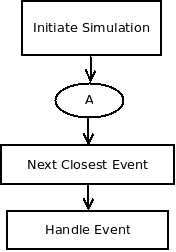
\includegraphics[scale=0.5]{f0.png}
    }
    \end{center}
\end{figure}

\begin{figure}[htp]
    \begin{center}
    \subfigure[Item leaves machining center]{
        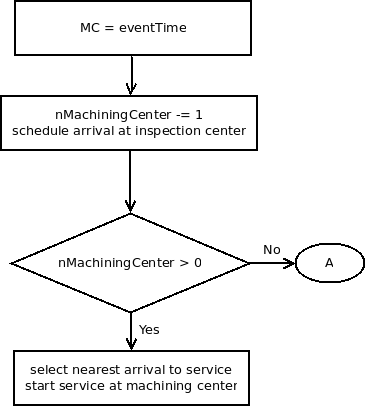
\includegraphics[scale=0.5]{f1.png}
    }
    \end{center}
\end{figure}

\newpage
\begin{figure}[htp]
    \begin{center}
    \subfigure[New item arrives machining center]{
        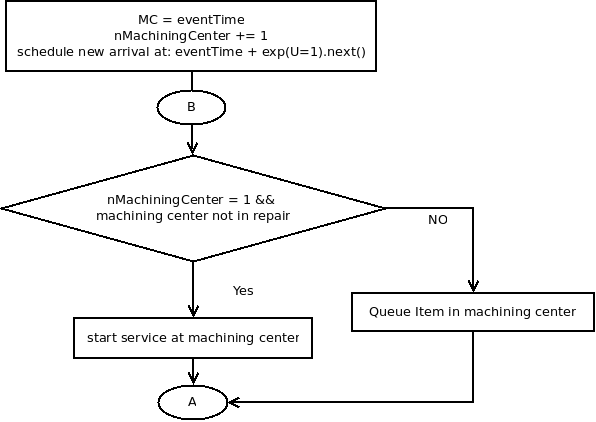
\includegraphics[scale=0.5]{f2.png}
    }
    \end{center}
\end{figure}

\begin{figure}[htp]
    \begin{center}
    \subfigure[Machining Center Breakdown]{
        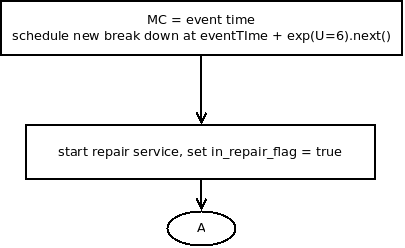
\includegraphics[scale=0.5]{f3.png}
    }
    \end{center}
\end{figure}

\newpage

\begin{figure}[htp]
    \begin{center}
    \subfigure[Machining Center Repaired]{
        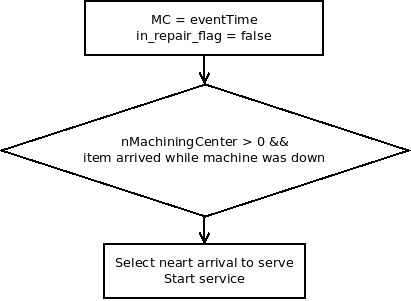
\includegraphics[scale=0.5]{f4.png}
    }
    \end{center}
\end{figure}

\begin{figure}[htp]
    \begin{center}
    \subfigure[Inspection Center Arrival]{
        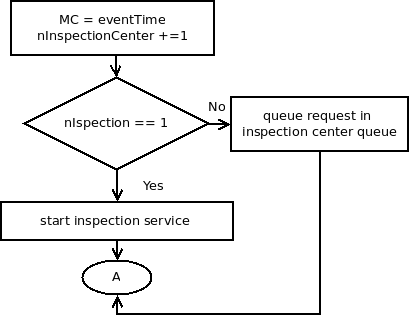
\includegraphics[scale=0.5]{f5.png}
    }
    \subfigure[Inspection Center Departure]{
        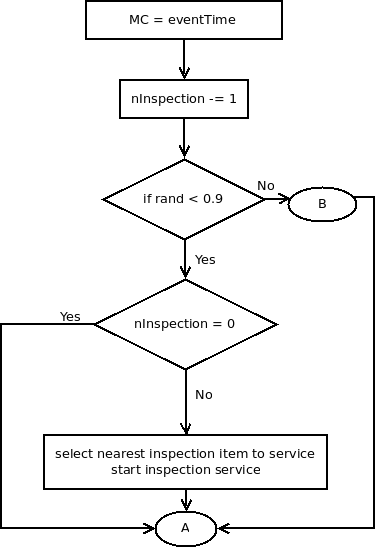
\includegraphics[scale=0.5]{f6.png}
    }
    \end{center}
\end{figure}

%%%%%%%%%%%%%%%%%%%%%%%%%%%%%%
%%%%%%%%%%%%%%%%%%%%%%%%%%%%%%
%%%%%%%%%%%%%%%%%%%%%%%%%%%%%%
\newpage
\section{Analysis}
    \subsection{LCG}
        \subsubsection{LCG Histogram}
            \begin{figure}[htp]
                \begin{center}
                \subfigure[LCG Histogram]{
                    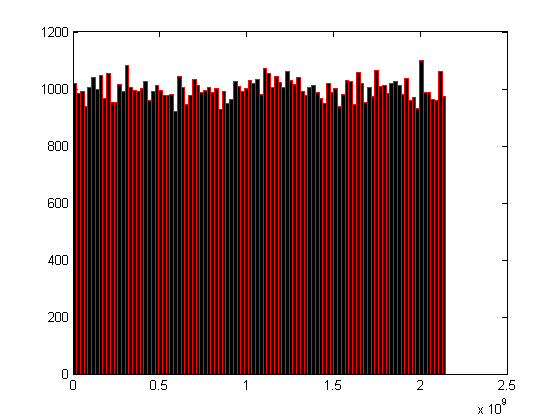
\includegraphics[scale=0.5]{lcg_hist.png}
                }
                \end{center}
            \end{figure}
        \subsubsection{LCG matlab generation script}
            \lstinputlisting{../analysis/1/sample.m}
        \subsubsection{Chi-Square Test}
            $D$ = 1.235240e+002

            $\alpha$ = 0.05

            Chi-square $(n=99,\alpha = 0.05)$ = 124

            So, this generator follows the uniform distribution.
    \subsection{Performance Metrics}
        \subsubsection{Inter-arrival times}
            \begin{itemize}
                \item Machining Center Inter-arrival times
                    \begin{itemize}
                        \item mean = 8.937310e-001
                        \item standard deviation = 9.035021e-001
                        \item Confidence-Interval = [ 8.755911e-001 , 9.118710e-001 ]
                    \end{itemize}
                    \begin{figure}[htp]
                        \begin{center}
                        \subfigure[Machining Center Inter-arrival times]{
                            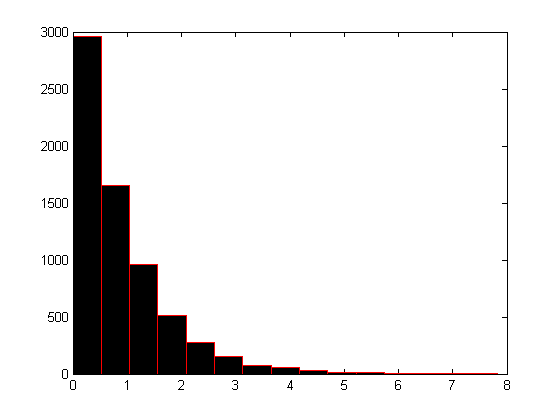
\includegraphics[scale=0.5]{../analysis/5/Images/machining_interarrival_time.png}
                        }
                        \end{center}
                    \end{figure}
                \item Inspection Center Inter-arrival times
                    \begin{itemize}
                        \item mean = 8.938989e-001
                        \item standard deviation = 7.429512e-001
                        \item Confidence-Interval = [ 8.789813e-001 , 9.088166e-001 ]
                    \end{itemize}
                    \begin{figure}[htp]
                        \begin{center}
                        \subfigure[Inspection Center Inter-arrival times]{
                            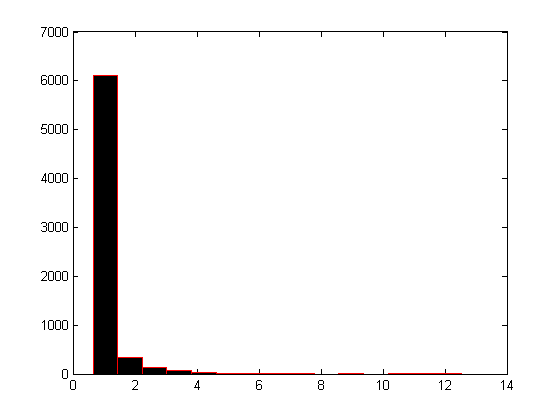
\includegraphics[scale=0.5]{../analysis/5/Images/inspection_interarrival_time.png}
                        }
                        \end{center}
                    \end{figure}
            \end{itemize}

        \newpage
        \subsubsection{Service times}
            \begin{itemize}
                \item Machining Center Service times
                    \begin{itemize}
                        \item mean = 6.748031e-001
                        \item standard deviation = 1.442324e-002
                        \item Confidence-Interval = [ 6.745135e-001 , 6.750927e-001 ]
                    \end{itemize}
                    \begin{figure}[htp]
                        \begin{center}
                        \subfigure[Machining Center Service times]{
                            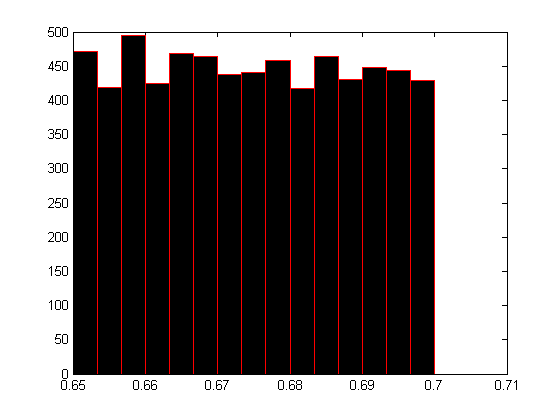
\includegraphics[scale=0.5]{../analysis/5/Images/machining_service_time.png}
                        }
                        \end{center}
                    \end{figure}
                \item Inspection Center Service times
                    \begin{itemize}
                        \item mean = 7.749589e-001
                        \item standard deviation = 1.443071e-002
                        \item Confidence-Interval = [ 7.746691e-001 , 7.752486e-001 ]
                    \end{itemize}
                    \begin{figure}[htp]
                        \begin{center}
                        \subfigure[Inspection Center Service times]{
                            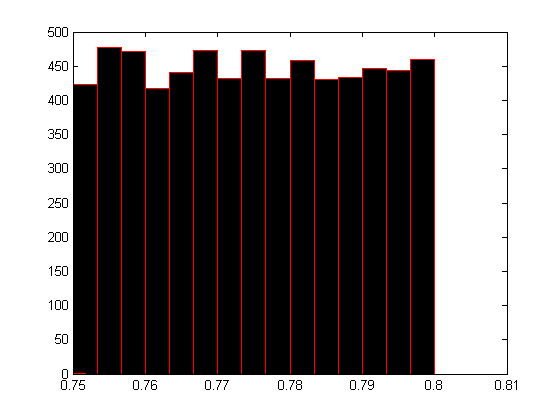
\includegraphics[scale=0.5]{../analysis/5/Images/inspection_service_time.png}
                        }
                        \end{center}
                    \end{figure}
            \end{itemize}

        \newpage
        \subsubsection{Response Times}
            \begin{itemize}
                \item mean = 5.937559e+000
                \item standard deviation = 4.959343e+000
                \item Confidence-Interval = [ 5.829767e+000 , 6.045352e+000 ]
            \end{itemize}
            \begin{figure}[htp]
                \begin{center}
                \subfigure[Response Time]{
                    \includegraphics[scale=0.5]{../analysis/5/Images/response_time.png}
                }
                \end{center}
            \end{figure}

        \newpage
        \subsubsection{Queue Length}
            \begin{itemize}
                \item Machining Center Queue
                    \begin{itemize}
                        \item Average Queue Length = 1.976038
                    \end{itemize}
                    \begin{figure}[htp]
                        \begin{center}
                        \subfigure[Machine Center Queue Length Over Time]{
                            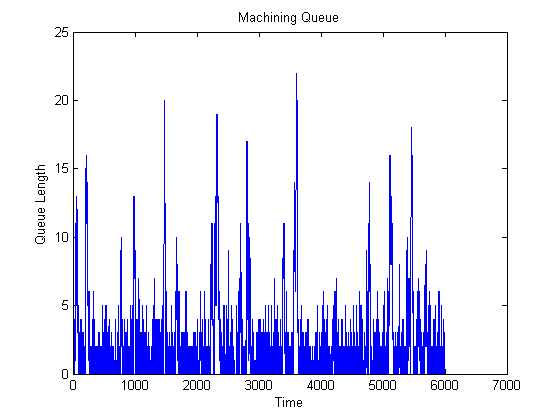
\includegraphics[scale=0.5]{../analysis/5/Images/machine_queue.png}
                        }
                        \end{center}
                    \end{figure}
                \item Inspection Center Queue
                    \begin{itemize}
                        \item Average Queue Length = 2.233752
                    \end{itemize}
                    \begin{figure}[htp]
                        \begin{center}
                        \subfigure[Inspection Center Queue Length Over Time]{
                            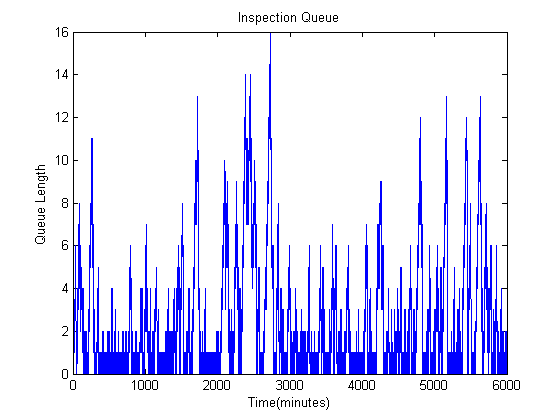
\includegraphics[scale=0.5]{../analysis/5/Images/inspection_queue.png}
                        }
                        \end{center}
                    \end{figure}
            \end{itemize}

        \newpage
        \subsubsection{Hourly Throughput}
            \begin{itemize}
                \item Average = 60.080000
                \item Standard Deviation = 0.571859
                \item Confidence-Interval = [ 5.978252e+001 , 6.037748e+001 ]
            \end{itemize}
            \begin{figure}[htp]
                \begin{center}
                \subfigure[Hourly Throughput]{
                    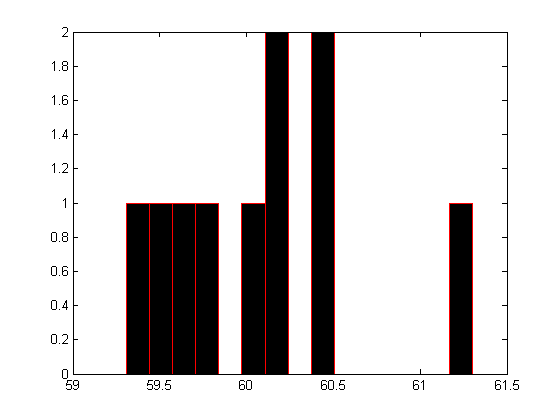
\includegraphics[scale=0.5]{../analysis/5/Images/hourly_throughput.png}
                }
                \subfigure[Hourly Throughput Over Time]{
                    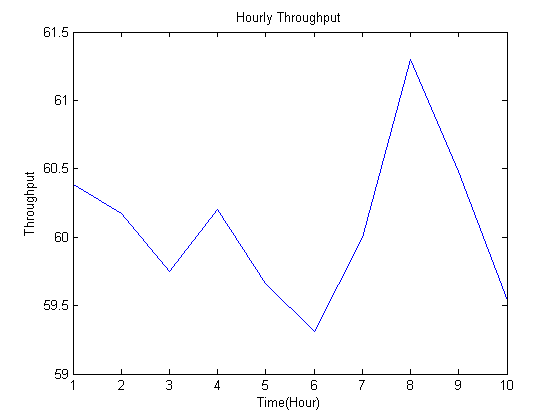
\includegraphics[scale=0.5]{../analysis/5/Images/hourly_throughput_vs_time.png}
                }
                \end{center}
            \end{figure}

    \newpage
    \subsection{Transient Removal}
        The Experiment has been repeated 10 times (replications) to get the next results
        \subsubsection{Moving Average}
            \begin{itemize}
                \item Moving Average results $=>$ the transient state is from hour 0 to 5.
            \end{itemize}
            \lstinputlisting{../analysis/6/Scripts/Moving_average.m}
            \begin{figure}[htp]
                \begin{center}
                \subfigure[Moving Averages with k=15]{
                    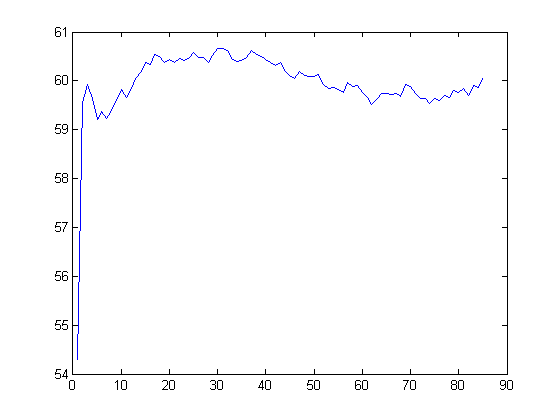
\includegraphics[scale=0.5]{../analysis/6/Images/moving_average_k_15.png}
                }
                \subfigure[Moving Averages with k=30]{
                    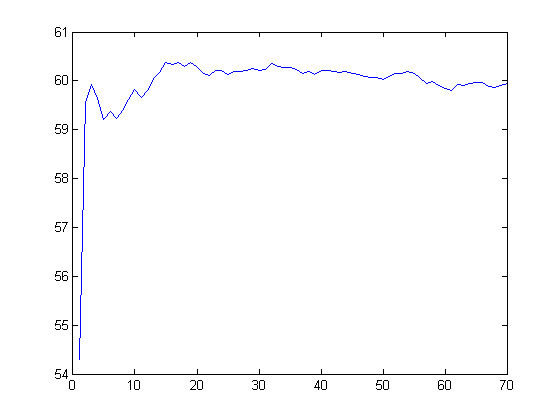
\includegraphics[scale=0.5]{../analysis/6/Images/moving_average_k_30.png}
                }
                \end{center}
            \end{figure}
        \newpage
        \subsubsection{Initial Data Removal}
            \begin{itemize}
                \item Initial data removal results are noisy.
            \end{itemize}
            \lstinputlisting{../analysis/6/Scripts/Initial_data_removal.m}
            \begin{figure}[htp]
                \begin{center}
                \subfigure[Initial data removal results]{
                    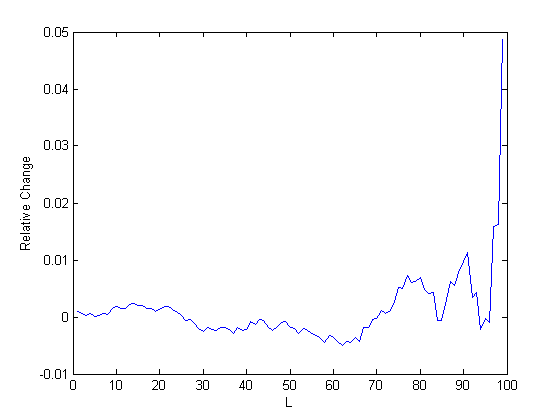
\includegraphics[scale=0.5]{../analysis/6/Images/initial_data_removal.png}
                }
                \end{center}
            \end{figure}

\newpage
\section{Selecting Stopping Criteria}
    The metric used for stopping criteria is The Hourly Throughput.

    Stopping creteria: confidence interval is 1\% from the mean.

    Estimated transient period from the hourly throughput curves through 10
    replications: 5 hours
    \\

    \subsection{Simuation Results}
        \begin{itemize}
            \item Simulation Duration = 100 hours
            \item 1 - alpha = 0.005
            \item Average = 60.080000
            \item Standard Diviation = 0.571859
            \item Confidence-Interval = [ 60.07891 , 60.08109 ]
        \end{itemize}

    \subsection{Conclusion}
        Since CI satisfies our Criteria (1\% from the mean) ,then 100 hour simulation is enough.

    \newpage
    \subsection{Recalculating performance metrics}
        \subsubsection{Inter-arrival times}
            \begin{itemize}
                \item Machining Center Inter-arrival times
                    \begin{itemize}
                        \item mean = 8.953830e-001
                        \item Standard deviation = 9.075272e-001
                        \item Confidence-Interval = [ 8.766737e-001 , 9.140923e-001 ]
                    \end{itemize}
                    \begin{figure}[htp]
                        \begin{center}
                        \subfigure[Machining Center Inter-arrival times]{
                            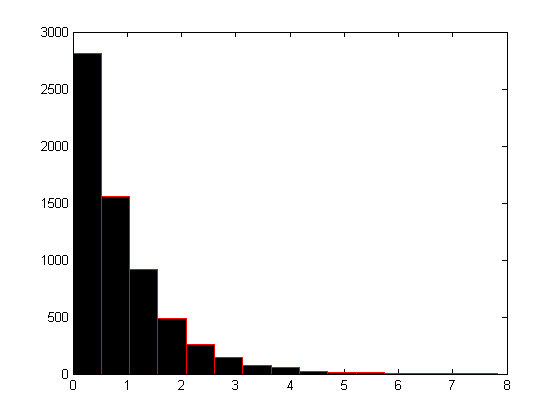
\includegraphics[scale=0.5]{../analysis/8/Images/machining_interarrival_time.png}
                        }
                        \end{center}
                    \end{figure}
                \item Inspection Center Inter-arrival times
                    \begin{itemize}
                        \item mean = 8.953662e-001
                        \item standard deviation = 7.293621e-001
                        \item Confidence-Interval = [ 8.803287e-001 , 9.104037e-001 ]
                    \end{itemize}
                    \begin{figure}[htp]
                        \begin{center}
                        \subfigure[Inspection Center Inter-arrival times]{
                            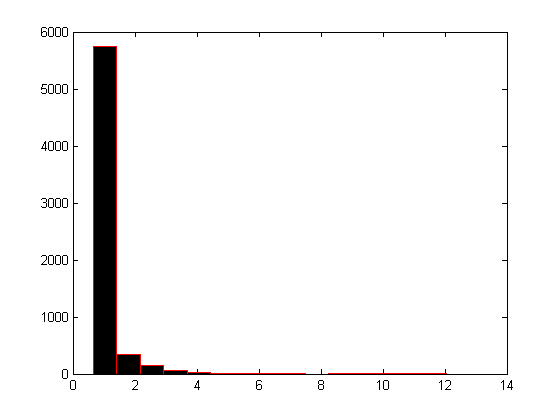
\includegraphics[scale=0.5]{../analysis/8/Images/inspection_interarrival_time.png}
                        }
                        \end{center}
                    \end{figure}
            \end{itemize}

        \newpage
        \subsubsection{Service times}
            \begin{itemize}
                \item Machining Center Service times
                    \begin{itemize}
                        \item mean = 6.748462e-001
                        \item standard deviation = 1.442515e-002
                        \item Confidence-Interval = [ 6.745488e-001 , 6.751437e-001 ]
                    \end{itemize}
                    \begin{figure}[htp]
                        \begin{center}
                        \subfigure[Machining Center Service times]{
                            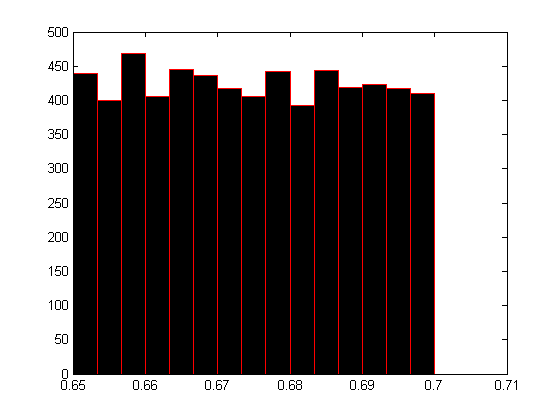
\includegraphics[scale=0.5]{../analysis/8/Images/maching_service_time.png}
                        }
                        \end{center}
                    \end{figure}
                \item Inspection Center Service times
                    \begin{itemize}
                        \item mean = 8.953662e-001
                        \item standard deviation = 7.293621e-001
                        \item Confidence-Interval = [ 8.803287e-001 , 9.104037e-001 ]
                    \end{itemize}
                    \begin{figure}[htp]
                        \begin{center}
                        \subfigure[Inspection Center Service times]{
                            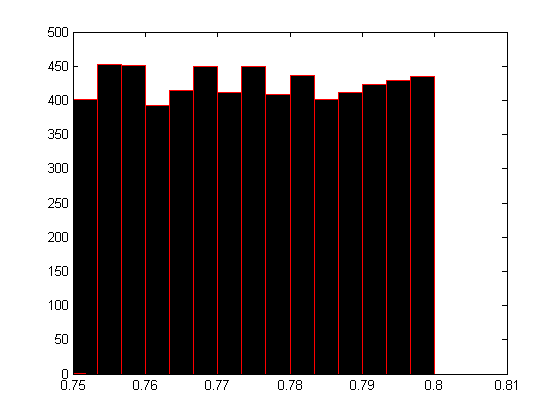
\includegraphics[scale=0.5]{../analysis/8/Images/inspection_service_time.png}
                        }
                        \end{center}
                    \end{figure}
            \end{itemize}

        \newpage
        \subsubsection{Response Times}
            \begin{itemize}
                \item mean = 5.937559e+000
                \item standard deviation = 4.959343e+000
                \item Confidence-Interval = [ 5.829767e+000 , 6.045352e+000 ]
            \end{itemize}
            \begin{figure}[htp]
                \begin{center}
                \subfigure[Response Time]{
                    \includegraphics[scale=0.5]{../analysis/8/Images/response_time.png}
                }
                \end{center}
            \end{figure}

        \newpage
        \subsubsection{Queue Length}
            \begin{itemize}
                \item Machining Center Queue
                    \begin{itemize}
                        \item Average Queue Length = 1.799588
                    \end{itemize}
                    \begin{figure}[htp]
                        \begin{center}
                        \subfigure[Machine Center Queue Length Over Time]{
                            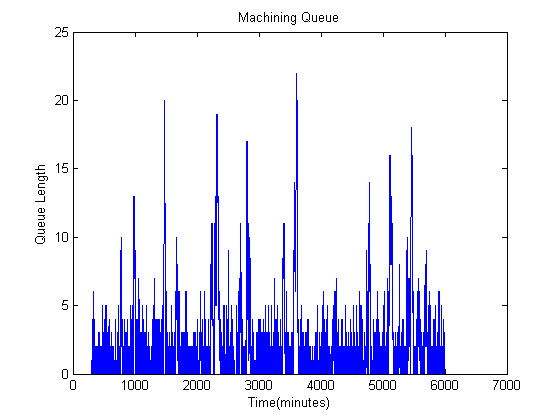
\includegraphics[scale=0.5]{../analysis/8/Images/maching_queue.png}
                        }
                        \end{center}
                    \end{figure}
                \item Inspection Center Queue
                    \begin{itemize}
                        \item Average Queue Length = 2.076659
                    \end{itemize}
                    \begin{figure}[htp]
                        \begin{center}
                        \subfigure[Inspection Center Queue Length Over Time]{
                            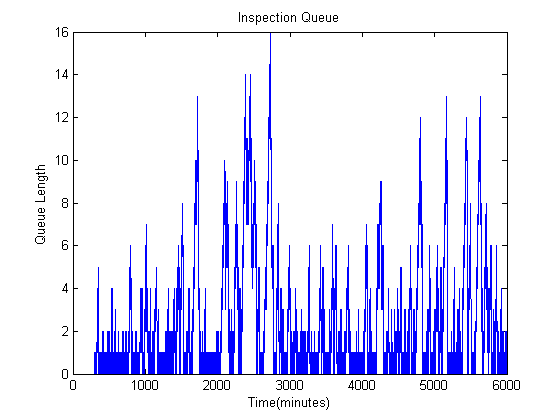
\includegraphics[scale=0.5]{../analysis/8/Images/inspection_queue.png}
                        }
                        \end{center}
                    \end{figure}
            \end{itemize}

        \newpage
        \subsubsection{Hourly Throughput}
            \begin{itemize}
                \item Average = 60.091489
                \item Standard Deviation = 0.666104
                \item Confidence-Interval = [ 6.009023e+001 , 6.009275e+001 ]
            \end{itemize}
            \begin{figure}[htp]
                \begin{center}
                \subfigure[Hourly Throughput]{
                    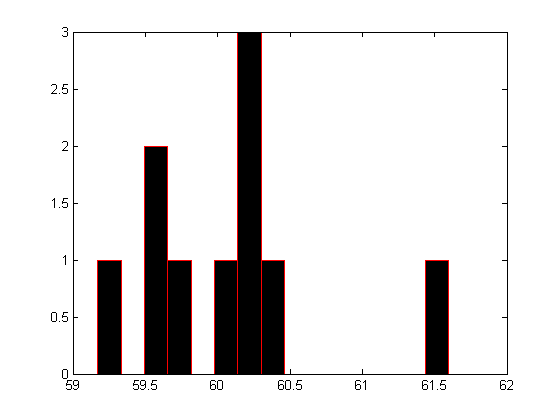
\includegraphics[scale=0.5]{../analysis/8/Images/hourly_throughput.png}
                }
                \subfigure[Hourly Throughput Over Time]{
                    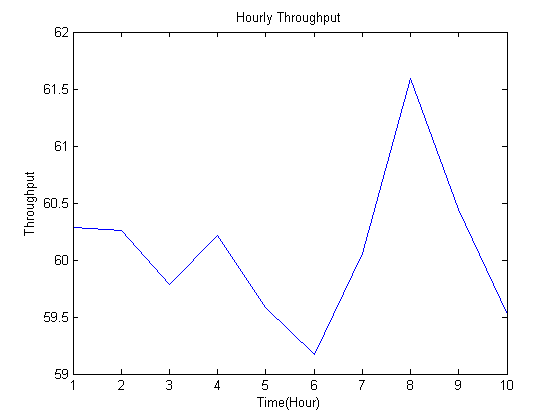
\includegraphics[scale=0.5]{../analysis/8/Images/hourly_throughput_vs_time.png}
                }
                \end{center}
            \end{figure}



                
                
% IF YOU'D RATHER TYPE THE CODE, OR HAVE A SMALLER BLOCK OF CODE, USE THIS:
%\begin{lstlisting}
%if(something)
%	do this
%else
%	do this
%\end{lstlisting}

%% THIS IS FROM A DIFFERENT CLASS, BUT DEMONSTRATES MATH MODE WELL
%%%%%%%%%%%%%%%%%%%%%%%%%%%%%%
\end{document}
